
%% bare_conf.tex
%% V1.4b
%% 2015/08/26
%% by Michael Shell
%% See:
%% http://www.michaelshell.org/
%% for current contact information.
%%
%% This is a skeleton file demonstrating the use of IEEEtran.cls
%% (requires IEEEtran.cls version 1.8b or later) with an IEEE
%% conference paper.
%%
%% Support sites:
%% http://www.michaelshell.org/tex/ieeetran/
%% http://www.ctan.org/pkg/ieeetran
%% and
%% http://www.ieee.org/

%%*************************************************************************
%% Legal Notice:
%% This code is offered as-is without any warranty either expressed or
%% implied; without even the implied warranty of MERCHANTABILITY or
%% FITNESS FOR A PARTICULAR PURPOSE! 
%% User assumes all risk.
%% In no event shall the IEEE or any contributor to this code be liable for
%% any damages or losses, including, but not limited to, incidental,
%% consequential, or any other damages, resulting from the use or misuse
%% of any information contained here.
%%
%% All comments are the opinions of their respective authors and are not
%% necessarily endorsed by the IEEE.
%%
%% This work is distributed under the LaTeX Project Public License (LPPL)
%% ( http://www.latex-project.org/ ) version 1.3, and may be freely used,
%% distributed and modified. A copy of the LPPL, version 1.3, is included
%% in the base LaTeX documentation of all distributions of LaTeX released
%% 2003/12/01 or later.
%% Retain all contribution notices and credits.
%% ** Modified files should be clearly indicated as such, including  **
%% ** renaming them and changing author support contact information. **
%%*************************************************************************


% *** Authors should verify (and, if needed, correct) their LaTeX system  ***
% *** with the testflow diagnostic prior to trusting their LaTeX platform ***
% *** with production work. The IEEE's font choices and paper sizes can   ***
% *** trigger bugs that do not appear when using other class files.       ***                          ***
% The testflow support page is at:
% http://www.michaelshell.org/tex/testflow/



\documentclass[conference]{IEEEtran}
% Some Computer Society conferences also require the compsoc mode option,
% but others use the standard conference format.
%
% If IEEEtran.cls has not been installed into the LaTeX system files,
% manually specify the path to it like:
% \documentclass[conference]{../sty/IEEEtran}





% Some very useful LaTeX packages include:
% (uncomment the ones you want to load)


% *** MISC UTILITY PACKAGES ***
%
%\usepackage{ifpdf}
% Heiko Oberdiek's ifpdf.sty is very useful if you need conditional
% compilation based on whether the output is pdf or dvi.
% usage:
% \ifpdf
%   % pdf code
% \else
%   % dvi code
% \fi
% The latest version of ifpdf.sty can be obtained from:
% http://www.ctan.org/pkg/ifpdf
% Also, note that IEEEtran.cls V1.7 and later provides a builtin
% \ifCLASSINFOpdf conditional that works the same way.
% When switching from latex to pdflatex and vice-versa, the compiler may
% have to be run twice to clear warning/error messages.






% *** CITATION PACKAGES ***
%
%\usepackage{cite}
% cite.sty was written by Donald Arseneau
% V1.6 and later of IEEEtran pre-defines the format of the cite.sty package
% \cite{} output to follow that of the IEEE. Loading the cite package will
% result in citation numbers being automatically sorted and properly
% "compressed/ranged". e.g., [1], [9], [2], [7], [5], [6] without using
% cite.sty will become [1], [2], [5]--[7], [9] using cite.sty. cite.sty's
% \cite will automatically add leading space, if needed. Use cite.sty's
% noadjust option (cite.sty V3.8 and later) if you want to turn this off
% such as if a citation ever needs to be enclosed in parenthesis.
% cite.sty is already installed on most LaTeX systems. Be sure and use
% version 5.0 (2009-03-20) and later if using hyperref.sty.
% The latest version can be obtained at:
% http://www.ctan.org/pkg/cite
% The documentation is contained in the cite.sty file itself.
\usepackage{graphicx}

\usepackage{enumitem}




% *** GRAPHICS RELATED PACKAGES ***
%
\ifCLASSINFOpdf
  % \usepackage[pdftex]{graphicx}
  % declare the path(s) where your graphic files are
  % \graphicspath{{../pdf/}{../jpeg/}}
  % and their extensions so you won't have to specify these with
  % every instance of \includegraphics
  % \DeclareGraphicsExtensions{.pdf,.jpeg,.png}
\else
  % or other class option (dvipsone, dvipdf, if not using dvips). graphicx
  % will default to the driver specified in the system graphics.cfg if no
  % driver is specified.
  % \usepackage[dvips]{graphicx}
  % declare the path(s) where your graphic files are
  % \graphicspath{{../eps/}}
  % and their extensions so you won't have to specify these with
  % every instance of \includegraphics
  % \DeclareGraphicsExtensions{.eps}
\fi
% graphicx was written by David Carlisle and Sebastian Rahtz. It is
% required if you want graphics, photos, etc. graphicx.sty is already
% installed on most LaTeX systems. The latest version and documentation
% can be obtained at: 
% http://www.ctan.org/pkg/graphicx
% Another good source of documentation is "Using Imported Graphics in
% LaTeX2e" by Keith Reckdahl which can be found at:
% http://www.ctan.org/pkg/epslatex
%
% latex, and pdflatex in dvi mode, support graphics in encapsulated
% postscript (.eps) format. pdflatex in pdf mode supports graphics
% in .pdf, .jpeg, .png and .mps (metapost) formats. Users should ensure
% that all non-photo figures use a vector format (.eps, .pdf, .mps) and
% not a bitmapped formats (.jpeg, .png). The IEEE frowns on bitmapped formats
% which can result in "jaggedy"/blurry rendering of lines and letters as
% well as large increases in file sizes.
%
% You can find documentation about the pdfTeX application at:
% http://www.tug.org/applications/pdftex





% *** MATH PACKAGES ***
%
%\usepackage{amsmath}
% A popular package from the American Mathematical Society that provides
% many useful and powerful commands for dealing with mathematics.
%
% Note that the amsmath package sets \interdisplaylinepenalty to 10000
% thus preventing page breaks from occurring within multiline equations. Use:
%\interdisplaylinepenalty=2500
% after loading amsmath to restore such page breaks as IEEEtran.cls normally
% does. amsmath.sty is already installed on most LaTeX systems. The latest
% version and documentation can be obtained at:
% http://www.ctan.org/pkg/amsmath





% *** SPECIALIZED LIST PACKAGES ***
%
%\usepackage{algorithmic}
% algorithmic.sty was written by Peter Williams and Rogerio Brito.
% This package provides an algorithmic environment fo describing algorithms.
% You can use the algorithmic environment in-text or within a figure
% environment to provide for a floating algorithm. Do NOT use the algorithm
% floating environment provided by algorithm.sty (by the same authors) or
% algorithm2e.sty (by Christophe Fiorio) as the IEEE does not use dedicated
% algorithm float types and packages that provide these will not provide
% correct IEEE style captions. The latest version and documentation of
% algorithmic.sty can be obtained at:
% http://www.ctan.org/pkg/algorithms
% Also of interest may be the (relatively newer and more customizable)
% algorithmicx.sty package by Szasz Janos:
% http://www.ctan.org/pkg/algorithmicx




% *** ALIGNMENT PACKAGES ***
%
%\usepackage{array}
% Frank Mittelbach's and David Carlisle's array.sty patches and improves
% the standard LaTeX2e array and tabular environments to provide better
% appearance and additional user controls. As the default LaTeX2e table
% generation code is lacking to the point of almost being broken with
% respect to the quality of the end results, all users are strongly
% advised to use an enhanced (at the very least that provided by array.sty)
% set of table tools. array.sty is already installed on most systems. The
% latest version and documentation can be obtained at:
% http://www.ctan.org/pkg/array


% IEEEtran contains the IEEEeqnarray family of commands that can be used to
% generate multiline equations as well as matrices, tables, etc., of high
% quality.




% *** SUBFIGURE PACKAGES ***
%\ifCLASSOPTIONcompsoc
%  \usepackage[caption=false,font=normalsize,labelfont=sf,textfont=sf]{subfig}
%\else
%  \usepackage[caption=false,font=footnotesize]{subfig}
%\fi
% subfig.sty, written by Steven Douglas Cochran, is the modern replacement
% for subfigure.sty, the latter of which is no longer maintained and is
% incompatible with some LaTeX packages including fixltx2e. However,
% subfig.sty requires and automatically loads Axel Sommerfeldt's caption.sty
% which will override IEEEtran.cls' handling of captions and this will result
% in non-IEEE style figure/table captions. To prevent this problem, be sure
% and invoke subfig.sty's "caption=false" package option (available since
% subfig.sty version 1.3, 2005/06/28) as this is will preserve IEEEtran.cls
% handling of captions.
% Note that the Computer Society format requires a larger sans serif font
% than the serif footnote size font used in traditional IEEE formatting
% and thus the need to invoke different subfig.sty package options depending
% on whether compsoc mode has been enabled.
%
% The latest version and documentation of subfig.sty can be obtained at:
% http://www.ctan.org/pkg/subfig




% *** FLOAT PACKAGES ***
%
%\usepackage{fixltx2e}
% fixltx2e, the successor to the earlier fix2col.sty, was written by
% Frank Mittelbach and David Carlisle. This package corrects a few problems
% in the LaTeX2e kernel, the most notable of which is that in current
% LaTeX2e releases, the ordering of single and double column floats is not
% guaranteed to be preserved. Thus, an unpatched LaTeX2e can allow a
% single column figure to be placed prior to an earlier double column
% figure.
% Be aware that LaTeX2e kernels dated 2015 and later have fixltx2e.sty's
% corrections already built into the system in which case a warning will
% be issued if an attempt is made to load fixltx2e.sty as it is no longer
% needed.
% The latest version and documentation can be found at:
% http://www.ctan.org/pkg/fixltx2e


%\usepackage{stfloats}
% stfloats.sty was written by Sigitas Tolusis. This package gives LaTeX2e
% the ability to do double column floats at the bottom of the page as well
% as the top. (e.g., "\begin{figure*}[!b]" is not normally possible in
% LaTeX2e). It also provides a command:
%\fnbelowfloat
% to enable the placement of footnotes below bottom floats (the standard
% LaTeX2e kernel puts them above bottom floats). This is an invasive package
% which rewrites many portions of the LaTeX2e float routines. It may not work
% with other packages that modify the LaTeX2e float routines. The latest
% version and documentation can be obtained at:
% http://www.ctan.org/pkg/stfloats
% Do not use the stfloats baselinefloat ability as the IEEE does not allow
% \baselineskip to stretch. Authors submitting work to the IEEE should note
% that the IEEE rarely uses double column equations and that authors should try
% to avoid such use. Do not be tempted to use the cuted.sty or midfloat.sty
% packages (also by Sigitas Tolusis) as the IEEE does not format its papers in
% such ways.
% Do not attempt to use stfloats with fixltx2e as they are incompatible.
% Instead, use Morten Hogholm'a dblfloatfix which combines the features
% of both fixltx2e and stfloats:
%
% \usepackage{dblfloatfix}
% The latest version can be found at:
% http://www.ctan.org/pkg/dblfloatfix




% *** PDF, URL AND HYPERLINK PACKAGES ***
%
%\usepackage{url}
% url.sty was written by Donald Arseneau. It provides better support for
% handling and breaking URLs. url.sty is already installed on most LaTeX
% systems. The latest version and documentation can be obtained at:
% http://www.ctan.org/pkg/url
% Basically, \url{my_url_here}.




% *** Do not adjust lengths that control margins, column widths, etc. ***
% *** Do not use packages that alter fonts (such as pslatex).         ***
% There should be no need to do such things with IEEEtran.cls V1.6 and later.
% (Unless specifically asked to do so by the journal or conference you plan
% to submit to, of course. )


% correct bad hyphenation here
\hyphenation{op-tical net-works semi-conduc-tor}


\begin{document}
%
% paper title
% Titles are generally capitalized except for words such as a, an, and, as,
% at, but, by, for, in, nor, of, on, or, the, to and up, which are usually
% not capitalized unless they are the first or last word of the title.
% Linebreaks \\ can be used within to get better formatting as desired.
% Do not put math or special symbols in the title.
\title{Principal Component Analysis and K-Means Clustering –
Biometrics- Project 2}


% author names and affiliations
% use a multiple column layout for up to three different
% affiliations
\author{\IEEEauthorblockN{Madhusudan Govindraju	}
\IEEEauthorblockA{
University of Florida\\
Email: madhusudangr@ufl.edu}
}

% conference papers do not typically use \thanks and this command
% is locked out in conference mode. If really needed, such as for
% the acknowledgment of grants, issue a \IEEEoverridecommandlockouts
% after \documentclass

% for over three affiliations, or if they all won't fit within the width
% of the page, use this alternative format:
% 
%\author{\IEEEauthorblockN{Michael Shell\IEEEauthorrefmark{1},
%Homer Simpson\IEEEauthorrefmark{2},
%James Kirk\IEEEauthorrefmark{3}, 
%Montgomery Scott\IEEEauthorrefmark{3} and
%Eldon Tyrell\IEEEauthorrefmark{4}}
%\IEEEauthorblockA{\IEEEauthorrefmark{1}School of Electrical and Computer Engineering\\
%Georgia Institute of Technology,
%Atlanta, Georgia 30332--0250\\ Email: see http://www.michaelshell.org/contact.html}
%\IEEEauthorblockA{\IEEEauthorrefmark{2}Twentieth Century Fox, Springfield, USA\\
%Email: homer@thesimpsons.com}
%\IEEEauthorblockA{\IEEEauthorrefmark{3}Starfleet Academy, San Francisco, California 96678-2391\\
%Telephone: (800) 555--1212, Fax: (888) 555--1212}
%\IEEEauthorblockA{\IEEEauthorrefmark{4}Tyrell Inc., 123 Replicant Street, Los Angeles, California 90210--4321}}




% use for special paper notices
%\IEEEspecialpapernotice{(Invited Paper)}




% make the title area
\maketitle

% As a general rule, do not put math, special symbols or citations
% in the abstract
\begin{abstract}
This papers gives a detailed report on how the problem statement has been understood and the steps and assumptions taken to solve the problem. In this paper, steps undertaken to implement Principal Component Analysis(PCA) and KMeans clustering for face recognition has been elaborated, along with their performance evaluations. The performance evaluations for PCA used in this paper are Receiver Operator Characteristics curve, Cumulative Match Characteristics Curve \& Genuine/Imposter Probablity Distributions. These plots are compared for different number of coefficients used in the PCA algorithm. The KMeans clustering algorithm has been implemented for gender a soft biometric classification example. Various external and internal characteristic indices have been used to evaluate the gender based soft biometric classification. 

\end{abstract}

% no keywords




% For peer review papers, you can put extra information on the cover
% page as needed:
% \ifCLASSOPTIONpeerreview
% \begin{center} \bfseries EDICS Category: 3-BBND \end{center}
% \fi
%
% For peerreview papers, this IEEEtran command inserts a page break and
% creates the second title. It will be ignored for other modes.
\IEEEpeerreviewmaketitle



\section{Introduction}
 The image which is used to test against the system's database of image is called the probe and the images which make up the database is called the gallery images. 
The complete project can be broadly divided in to two; one, PCA for face detection step ;two; kmeans for soft biometric classification. 

Principal Component Analysis(PCA) was first used for face recognition in \cite{PcaForFaceFirst}, most algorithms available perform matching in two steps ; step one, project the images into the subspace; step two, measure the similarity and classify in the subspace. In \cite{PcaForFaceFirst} they demonstrate "that the any particular face can be represented in a best coordinate system that they term eigenpicture". The method to calculate this eigen picture is described in detail in the subsection {\sl"Principal Component Analysis: EigenFaces method"} under the Method of Implementation. The performance of the system is evaluated using the CMC curve, ROC curve, genuine and imposter distribution curves. The curves obtained for the system implemented are described in detail in later sections. 

Clustering is an unsupervised method. In other words, the labels are not given to the clustering algorithm. The clustering algorithm tries to find a common point and classifies the data.The KMeans clustering is a flat clustering approach. It is initialized with a local centroid and iteratively tries to minimize the cost function. One of the important step in data clustering is feature selection. So using more information that describes the data perfectly helps in producing a better set of clusters.  The cost function and the steps to iteratively minimize the objective function  is described in detail in the subsection {\sl"K Means Clustering"}, under the "Methods of Implementation" section. The results of clustering algorithm is verified for correctness using internal validity criteria and external validity criteria. In out implementation we check the validity using the Calinski-Harabasz Index, Davies-Bouldin Index and Silhouette Width Criterion Index as the internal validity criteria; F-measure and Entropy as external validity criteria.

\section{The Data}

\begin{figure}[h!]
\centering
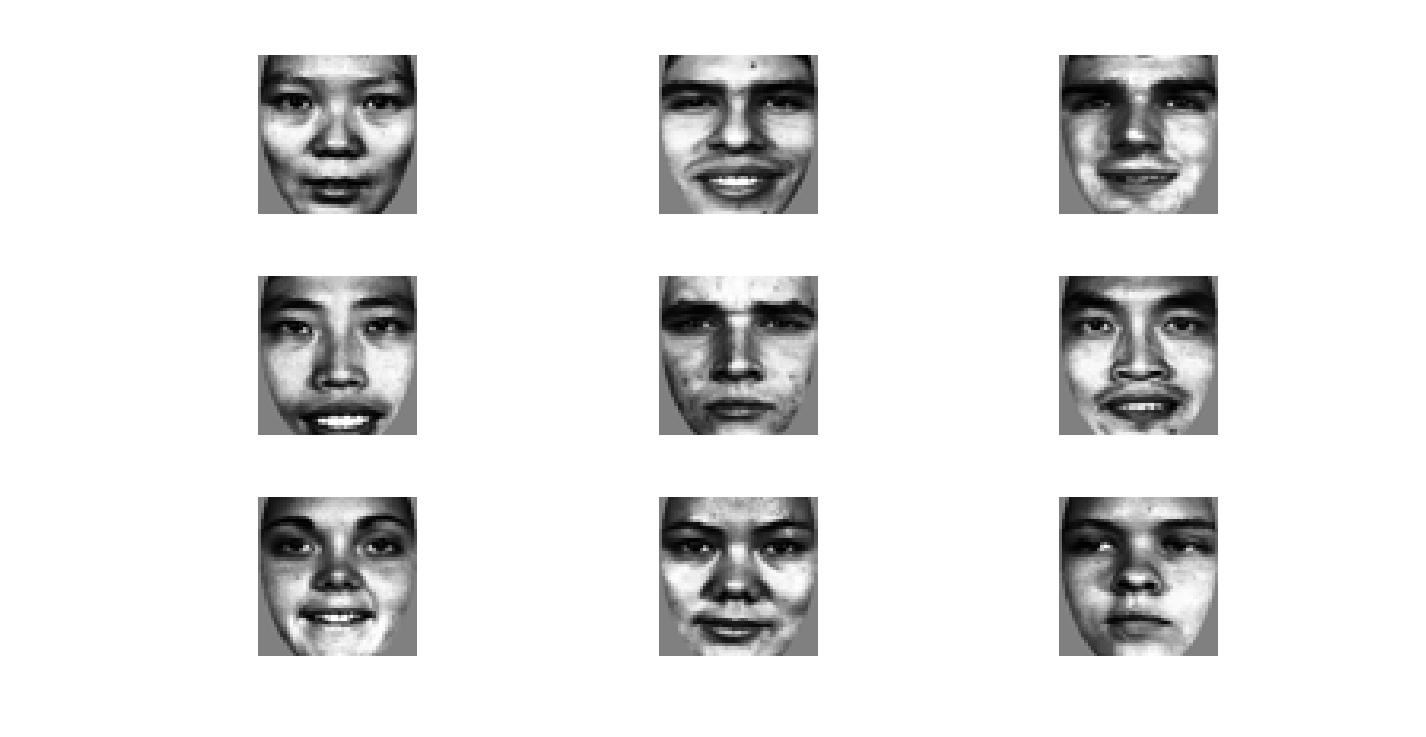
\includegraphics[scale=0.15]{GallerySample.jpg}
\caption{Sample images From the GallerySet }
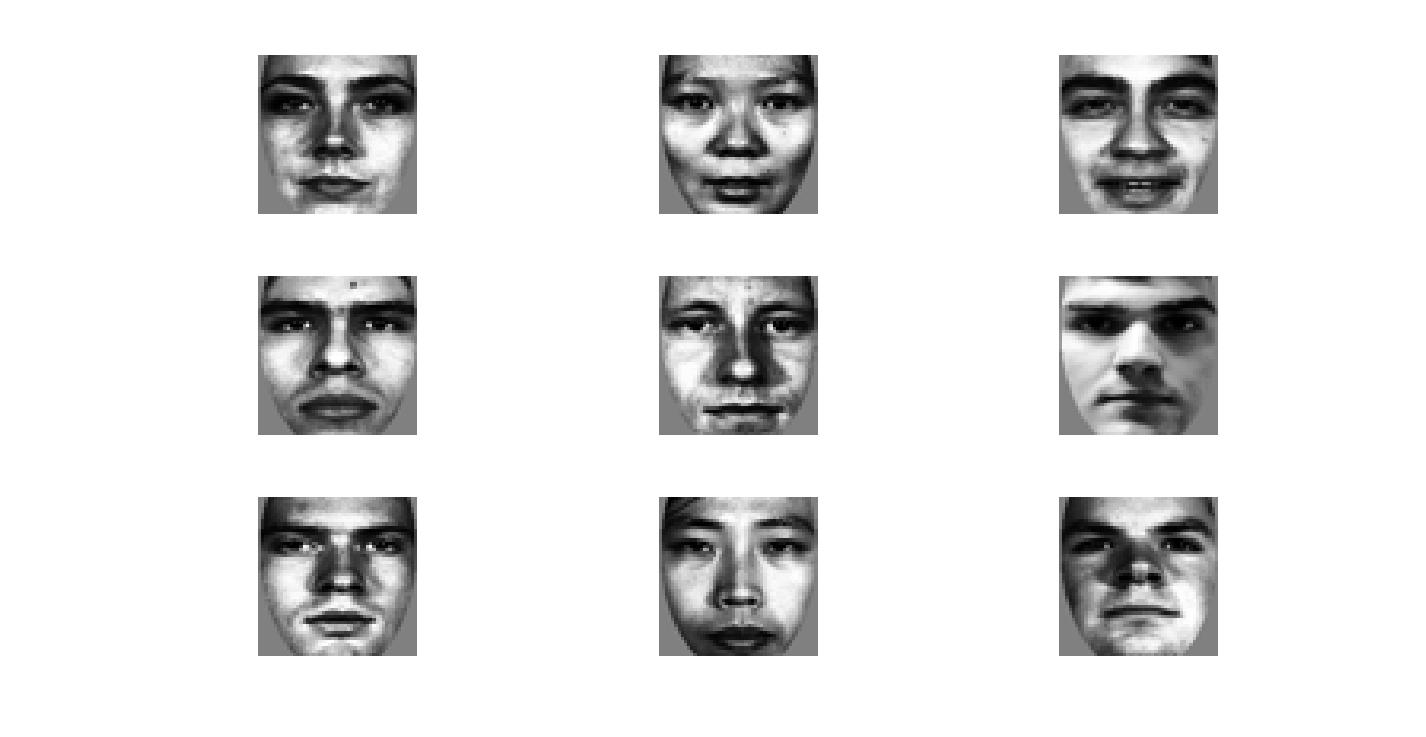
\includegraphics[scale=0.15]{ProbeSample1.jpg}
\caption{Sample images From the ProbeSet}
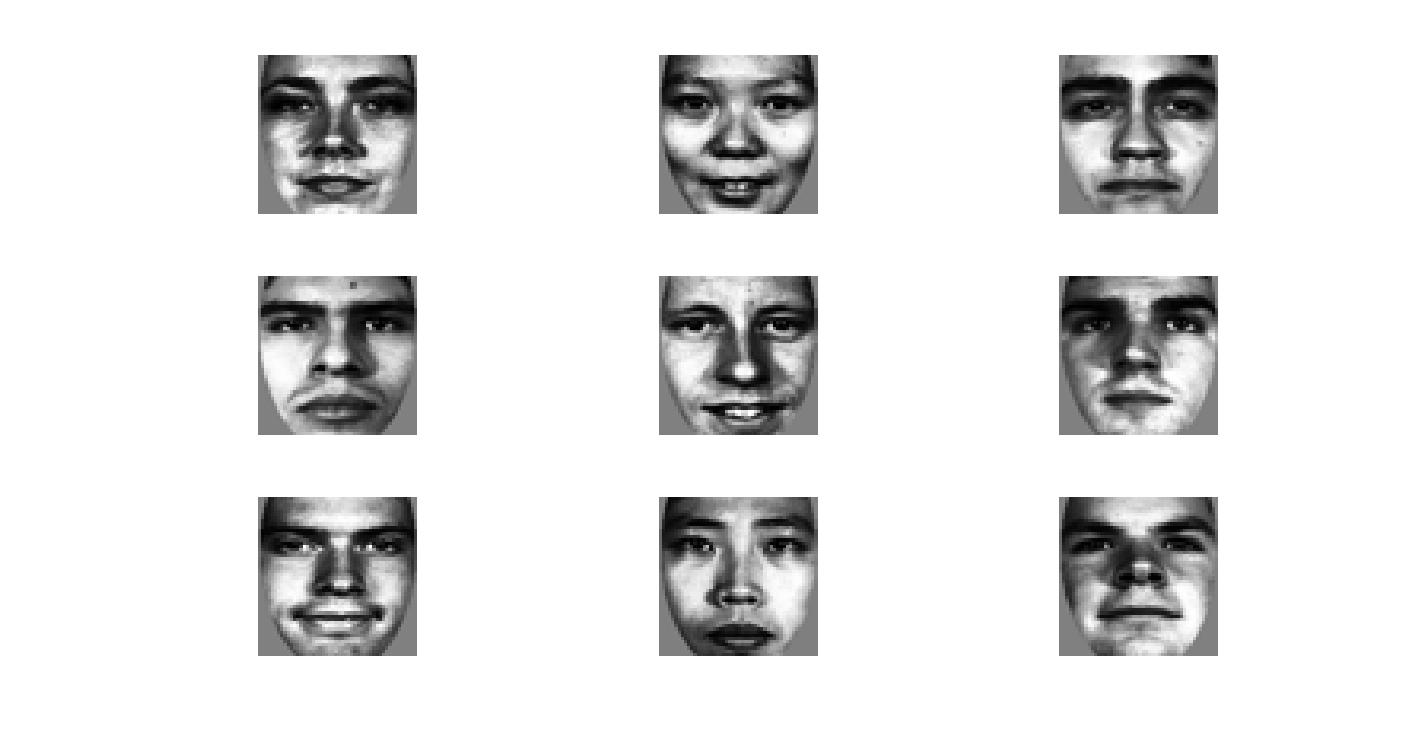
\includegraphics[scale=0.15]{ProbeSample2.jpg}
\caption{Sample images From the ProbeSet}
\label{fig:sampleGallery}
\end{figure}
The input data is a set of 3 images from 100 individuals. A total of 300 images. Each input image is of size 50x50 and is of uint8 type. A sample of the images from the gallery  and probe set is shown in the figure \ref{fig:sampleGallery}. The data set is divided into Gallery set and Probe Set. The first image from each individual is given as the gallery image and it corresponds to the training data. The other two images from each individual is given as the probe images and it corresponds to the testing data. We train the PCA for Face recognition algorithm with these 100 gallery images. We test the algorithm with the 200 probe images.  From the figure \ref{fig:sampleGallery} we can understand that the input faces are preprocessed and ready to use. If the images are not preprocessed we need to center \& align the faces, apply illumination normalization effects to the database before using it in out system. 

Before using the data we have to reshape the image into a 2500x1vector. This is in accordance with the PCA algorithm mentioned in the paper \cite{PcaForFaceFirst}. For eg., the gallery images will be aligned into a 2500x100 vector , where each column is a different sample.


\section{Method of Implementation}
The steps to implement the PCA for face detection and the Kmeans for gender classification are explained in the following subsection. 



\subsection{Principal Component Analysis: EigenFaces method}
The steps to calculate the Eigen faces and the corresponding coefficients is as follows \cite{PcaForFaceFirst},
\begin{enumerate}[label=(\alph*)]
\item The face images are loaded from the data sets and rearranged to form a vector of size 2500xM where M is the number of images. Each image was originally 50x50 which has been rearranges to a one dimensional vector 2500x1, This is $\Gamma$
\item Find the mean image $\Psi$
\item Subtract the mean image from every image to get the $\Phi(i)$ and we group all the $\Phi(i....m)$ together to get the matrix A.
\item Now if we find the covariance of A to find the eigenvectors and eigenvalues . The resulting matrix is very large, instead of finding the covariance matrix $ A \times A^{T} $ we find the matrix $ A^{T}\times A $ and  then compute the eigenvectors($v_{i}$) 
$$
        A^{T}Av_{i} = \mu_{i}v_{i}	
$$
\item We sort the eigenvalues($\mu$) in descending order and then pick the top 3( to top 100 in steps) eigenvectors corresponding to the top 3 (to top 100 in steps) eigenvalues, and calculate the eigenvectors$u_{i}$ of the $AA^{T}$ matrix using the following formula,
$$
u_{i} = Av_{i}
$$
\item This $u_{i}$ vector is rearranged in a $50\times50$ matrix to get the eigenfaces. 
\item The weights are calculated by multiplying the top N required eigenfaces with the matrix $A$.
\end{enumerate}
\begin{figure}[h!]
\centering
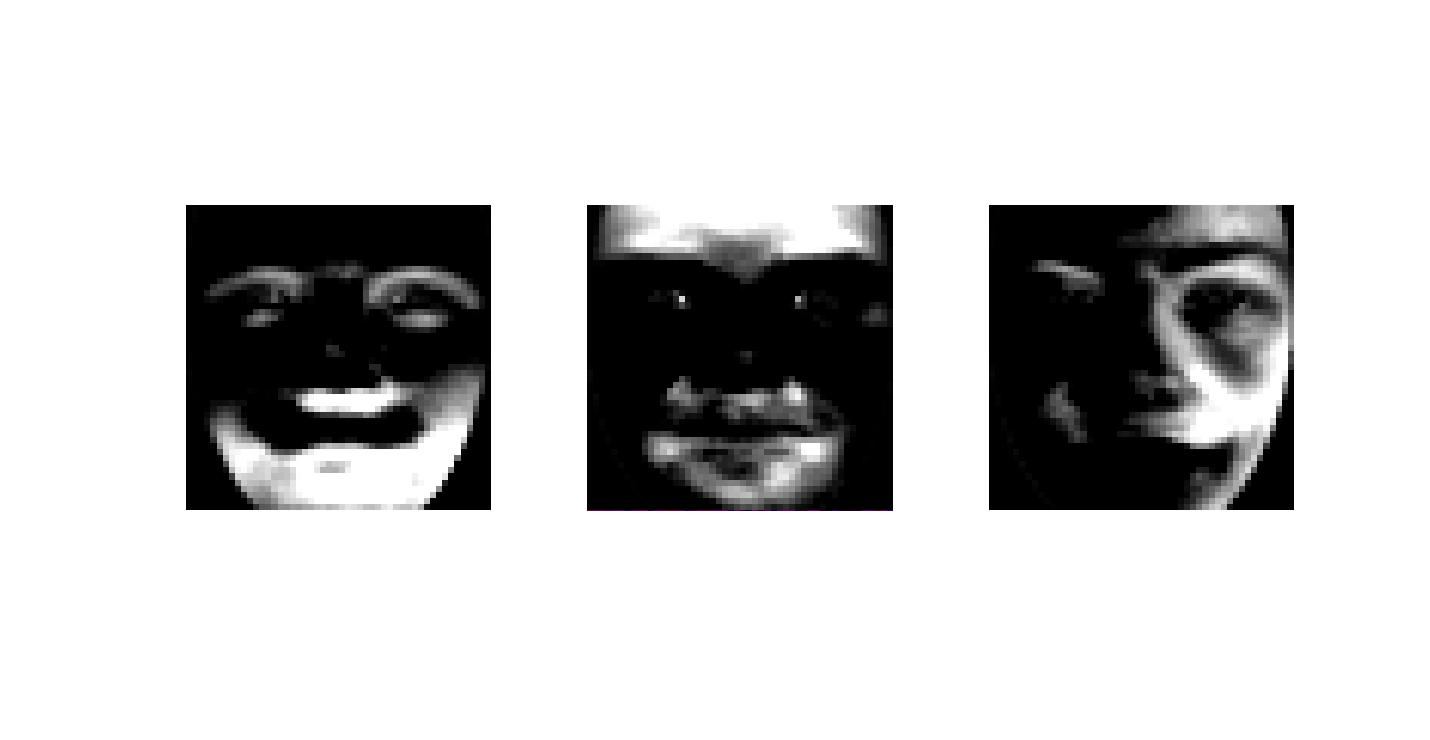
\includegraphics[scale=0.15]{top3eigenfaces.jpg}
\caption{Top 3 Eigen faces }
\label{fig:top3}
\end{figure}

Using the top 3 eigen vectors we  rearrange the vectors into images of size 50x50 and that is available in the figurre \ref{fig:top3}. The first principal component or the first eigen vector corresponds to illumination varianec. And thus to normalize the effect of illumination, experts mostly drop the first eigen vector.

\subsection{K Means Clustering}

In this type of clustering we start with a random point or centroid in this case and iteratively loop to proceed in the direction to reduce the cost function. The disadvantage of this algorithm is that we may reach a local minimum and it may not be anywhere near the global minimum, and if we don't know the data's external properties such as the labels it is impossible to find out the validity of the clusters. From the problem statement we have the labels so we will be able to check the internal and external cluster validity index to evaluate the clusters. The procedure to cluster the data is elaborated in steps below. 
\begin{enumerate}[label=(\alph*)]
\item It is understood that we need to cluster the given input data of 300 images into 2 clusters, Male and Female. So K = 2
\item We run the following steps for different centroid seeds, such as zero vector \& first two input data. ( The best performance was obtained with zero vector and hence we finalized with this as the seed)
\item With the seeded mean we populate the membership matrix using the membership function shown in the figure \ref{fig:MembershipFunction}. We use euclidean distance as the similarity measure between the vectors $x_i \& v_j$ in every step. 

\begin{figure}[h!]
\centering
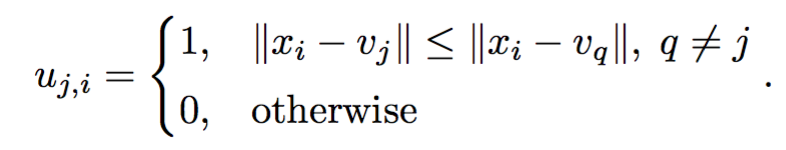
\includegraphics[scale = 0.5]{MembershipFunction}
\caption{Membership Function}
\label{fig:MembershipFunction}
\end{figure}

\begin{figure}[h!]
\centering
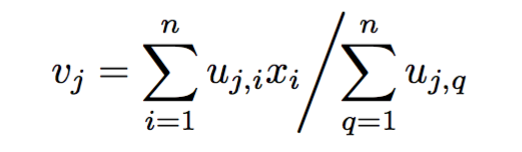
\includegraphics[scale=0.5]{UpdateMean}
\caption{ Update Mean Function}
\label {fig:UpdateMean}
\end{figure}

\begin{figure}[h!]
\centering
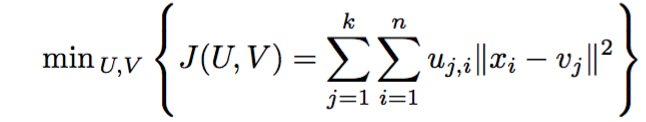
\includegraphics[scale=0.5]{ObjectiveFunction}
\caption{ Objective Function}
\label {fig:ObjectiveFunction}
\end{figure}

\item After populating the membership matrix with the membership function, we recalculate the mean for the new members as portrayed by the new membership matrix. We use the formula shown in figure \ref{fig:UpdateMean} to update the mean. 
\item After a new mean or the new centroid has been calculated the Cost is calculated using the formula in figure \ref{fig:ObjectiveFunction}

\item We repeat the steps 3 4 5 till J or the cluster centroids/mean does not change

\end{enumerate}

\subsubsection{\textbf{Centroid Seed Choice}}
In the case mentioned above we choose the mean to be zero vector, but in actual scenario we can let the centroid be any vector in the input sample space. This leads us to understand that the performance of the K means algorithm will vary for different starting centroids.
The K means's disadvantage is it minimizes the objective function to reach the local minimum and not the global minimum. Hence the seed for the centroid is an important factor to achieve proper cluster validity. 
The seed decides the following the maximum number of iterations required to reach the local minimum, hence reaching a poor convergence rate and hence produce sub optimal clusterings
 Will result in suboptimal final cost. (Final J)

Another known method is to initialize the parameters in a gaussian mixture model. \cite{BishopPattern}

%\subsubsection{\textbf{Validity Criteria}}
%\begin{enumerate}[label=(\alph*)]
%\item Internal
%\item External
%\end{enumerate}


\section{Evaluations}
This section explains the various steps taken to evaluate the systems described above. \\
\textbf{PCA}
\begin{enumerate}
\item With the 200 probe images and 100 gallery images, we calculate the {\sl Similarity Matrix} of size 200x100 where every image from the probe set is compared with the gallery set to get a similarity measure and this similarity measure is used to populate the similarity matrix. Since our similarity measure is euclidean distance the lesser the value the more similar it is. 
\item We can obtain the genuine score from the diagonal elements and the rest constitute the imposter scores. The genuine imposter distributions are the probability distributions for the genuine and imposter matches in the dataset. The area shared by both the curves gives a measure of how close the imposter and genuine comparisons are. A system that separates this genuine and imposter curves the max is said to perform better than the others.
\item The cumulative match characteristics curve gives the rank-t identification rate. CMC curve gives us the least rank to implement to get max recognition rate. Thus if this is achieved sooner the better is the system's performance. 
\item The receiver operator characteristics curve(roc) is calculated using the false match rate and the (1-false non match rate). The false match rate is the number of imposters that are lesser than the threshold divided by the number of imposter comparisons . The false non match rate is the number of genuine scores greater than the threshold divide by the number of genuine comparisons. The ares under the curve should be close to 100\% the higher the area under the curve the better is the performance.
\item From the images \ref{top10Coef} \ref{top20Coef} \ref{top30Coef} \ref{top40Coef} \ref{top50Coef} \ref{top60Coef} \ref{top70Coef} \ref{top80Coef} \ref{top90Coef} \ref{top100Coef}, we can understand that there is not much change in performance of the system as the number of coefficients increase from 10 to 100. Or the major variance of the dataset is available in the top 10 eigenvectors and hence incorporating them gives us the optimal performance that can be obtained from this input data. But as a whole as there is not much variation in the plots.

\begin{figure*}[h!]
\centering
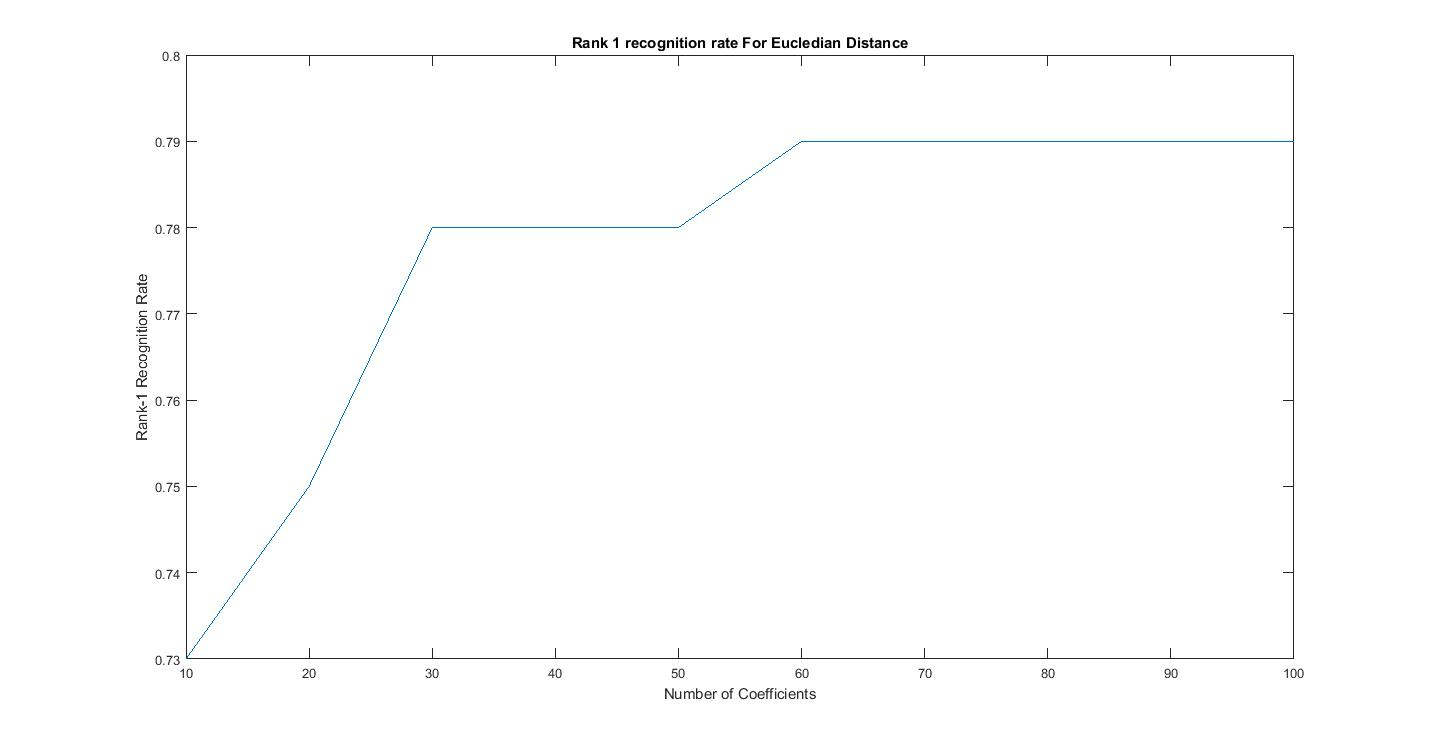
\includegraphics[width=20cm]{Rank1recognitionRateEuclideanDist.jpg}
\caption{Rank 1 Recognition Rate vs Number of Coeffecients}
\label {fr1VScoeff}
\end{figure*}
\item Even though there was not much overall difference in the above mentioned figures, from figure \ref{fr1VScoeff} we can infer that we need at least 60 coefficients for obtaining the best rank1 recognition rate.  Rank 1 recognition rate gives the accuracy for the system as a whole when keeping the highest threshold possible. Keeping a higher threshold corresponds to moving the threshold towards the left in the genuine and imposter distribution graphs. Moving the threshold towards the left leads to reducing the number of false matches and increasing the number of true negatives. Increasing the true negatives is going to reduce the accuracy of the system and reducing the false positives is going to increase the accuracy of the system. We have negotiate between these to get the best operating point. For achieving this best optimal operating point the rank 1 recognition rate gives us a measure of how high the threshold can be moved without reducing the accuracy of the system. This curve along with CMC curve can be used to compare different systems. 
%\begin{figure*}
%\centering
%\includegraphics[scale = 0.5]{}
%\caption{The Performance Characteristics for top Coeccefients}
%\label{top10Coef}
%\end{figure}

\begin{figure*}
\centering
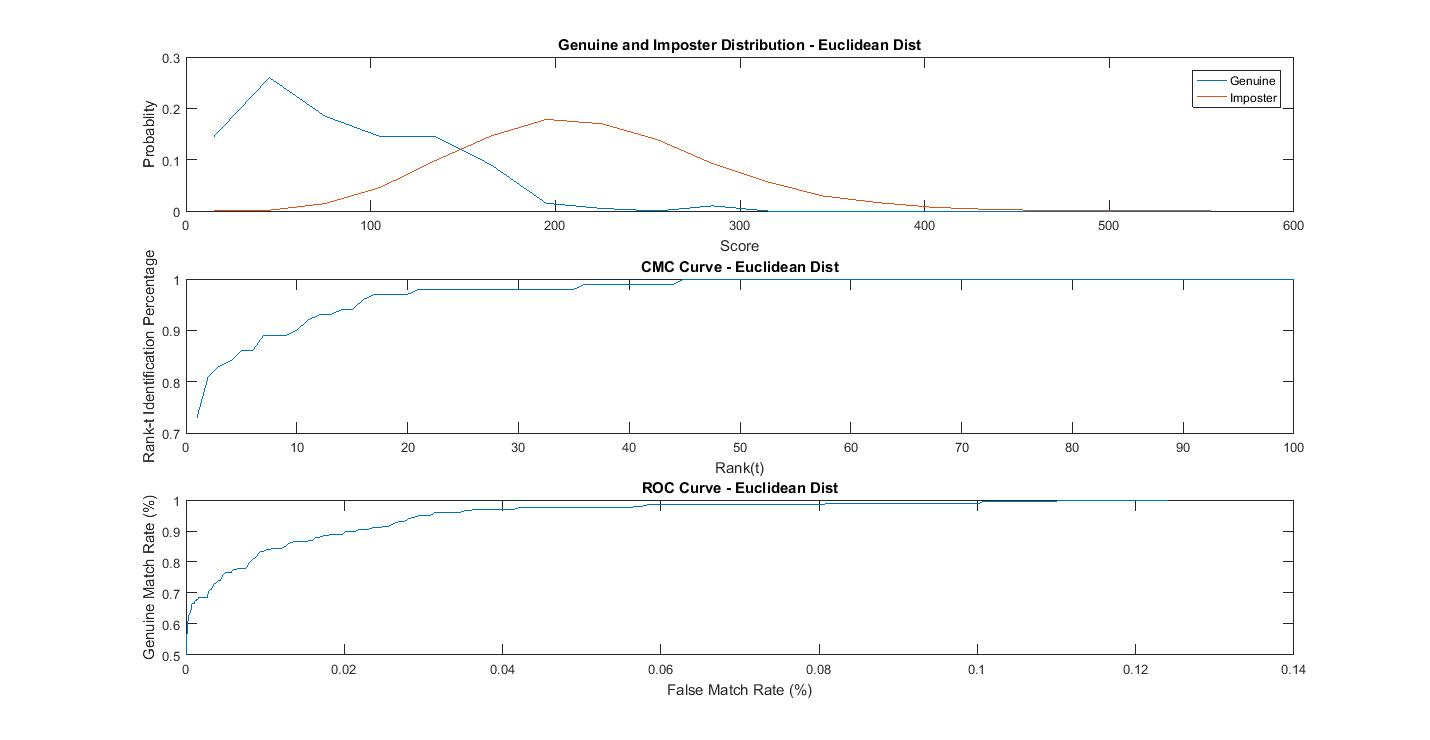
\includegraphics[width=20cm]{forTop10Coeffecients.jpg}
\caption{The Performance Characteristics for top 10 Coefficients}
\label{top10Coef}
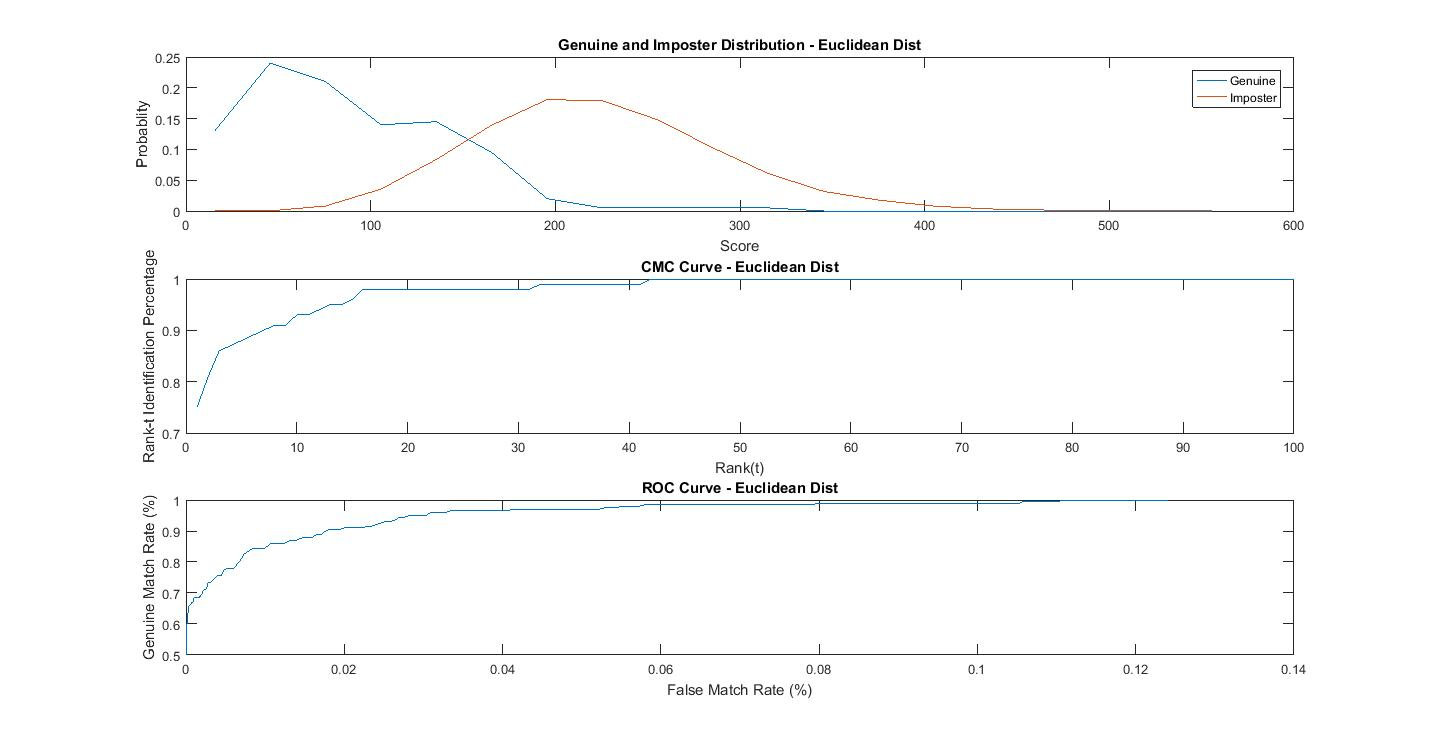
\includegraphics[width=20cm]{forTop20Coeffecients.jpg}
\caption{The Performance Characteristics for top 20 Coefficients}
\label{top20Coef}
\end{figure*}


\begin{figure*}
\centering
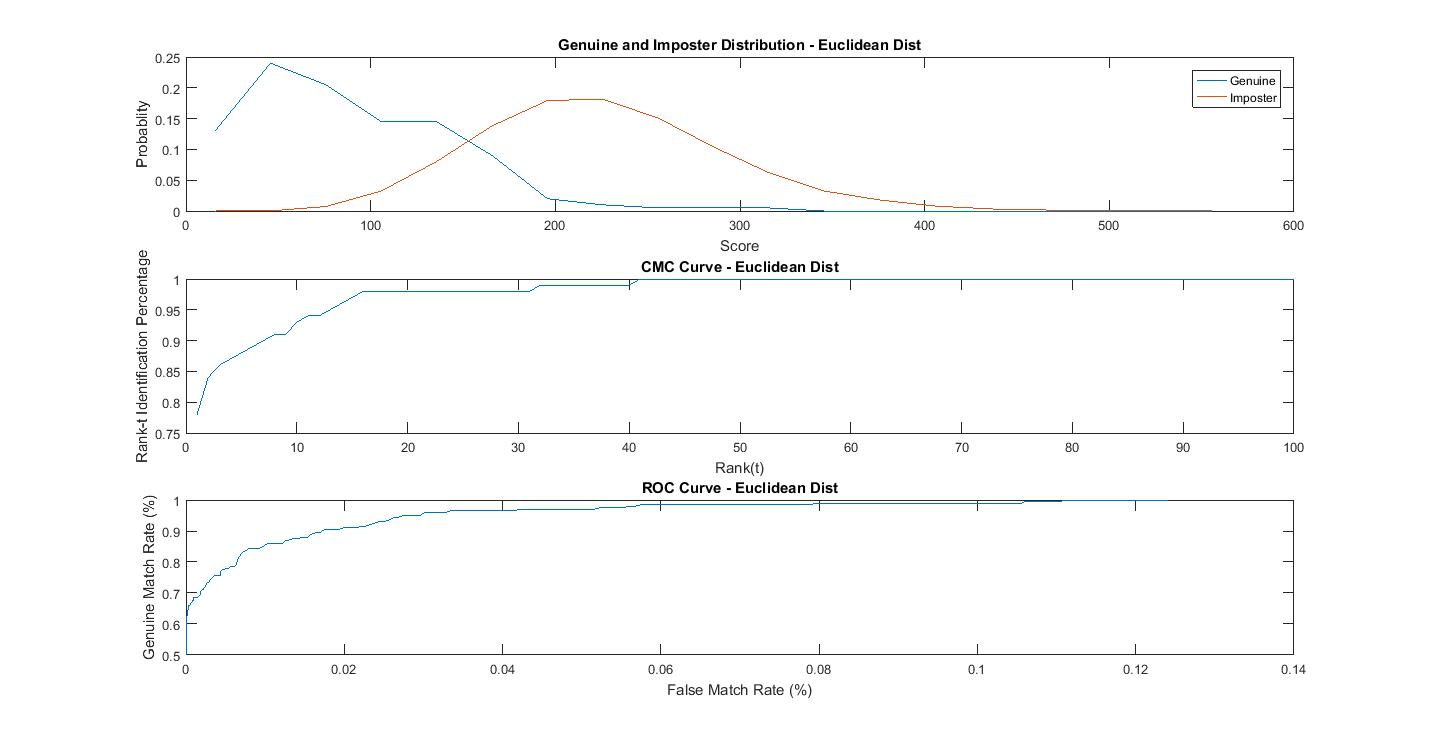
\includegraphics[width=20cm]{forTop30Coeffecients.jpg}
\caption{The Performance Characteristics for top 30 Coefficients}
\label{top30Coef}
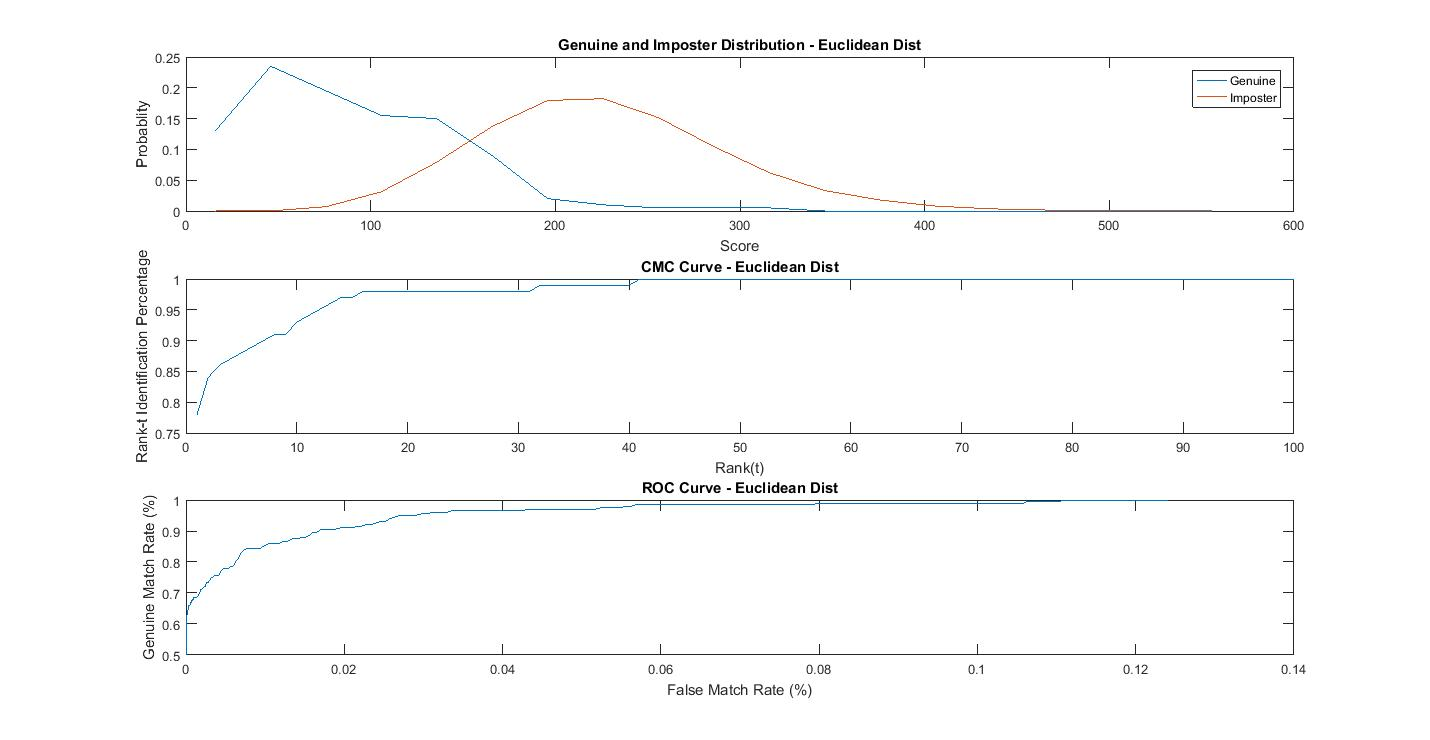
\includegraphics[width=20cm]{forTop40Coeffecients.jpg}
\caption{The Performance Characteristics for top 40 Coefficients}
\label{top40Coef}
\end{figure*}

\begin{figure*}
\centering
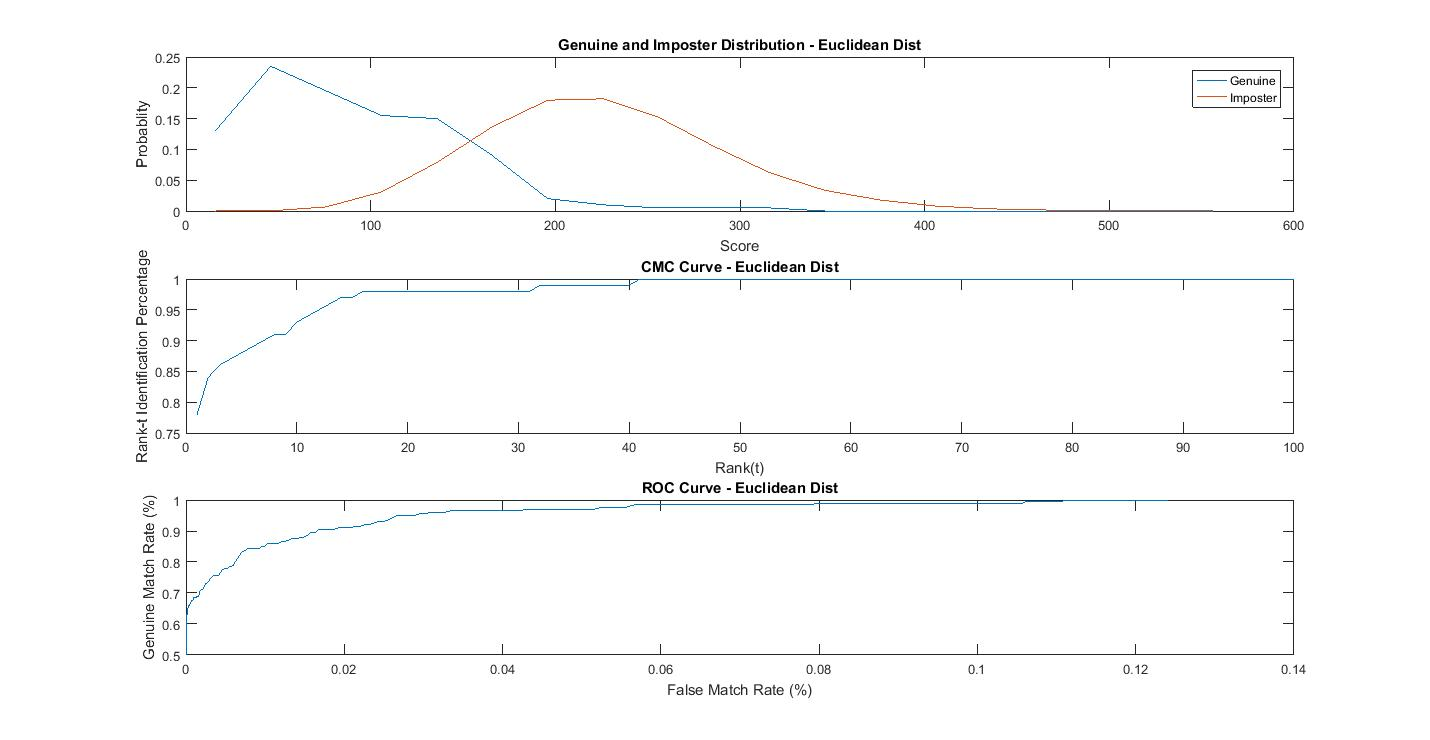
\includegraphics[width=20cm]{forTop50Coeffecients.jpg}
\caption{The Performance Characteristics for top 50 Coefficients}
\label{top50Coef}
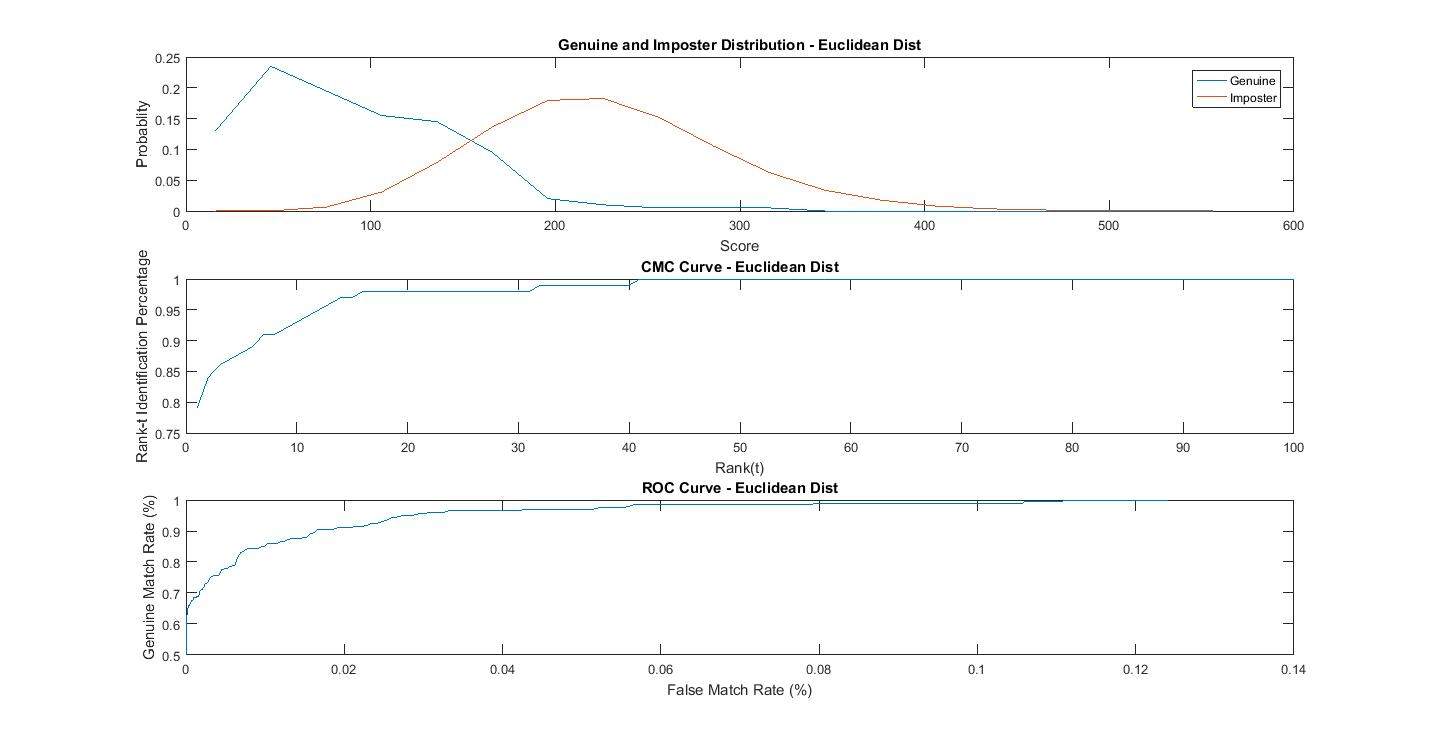
\includegraphics[width=20cm]{forTop60Coeffecients.jpg}
\caption{The Performance Characteristics for top 60 Coefficients}
\label{top60Coef}
\end{figure*}


\begin{figure*}
\centering
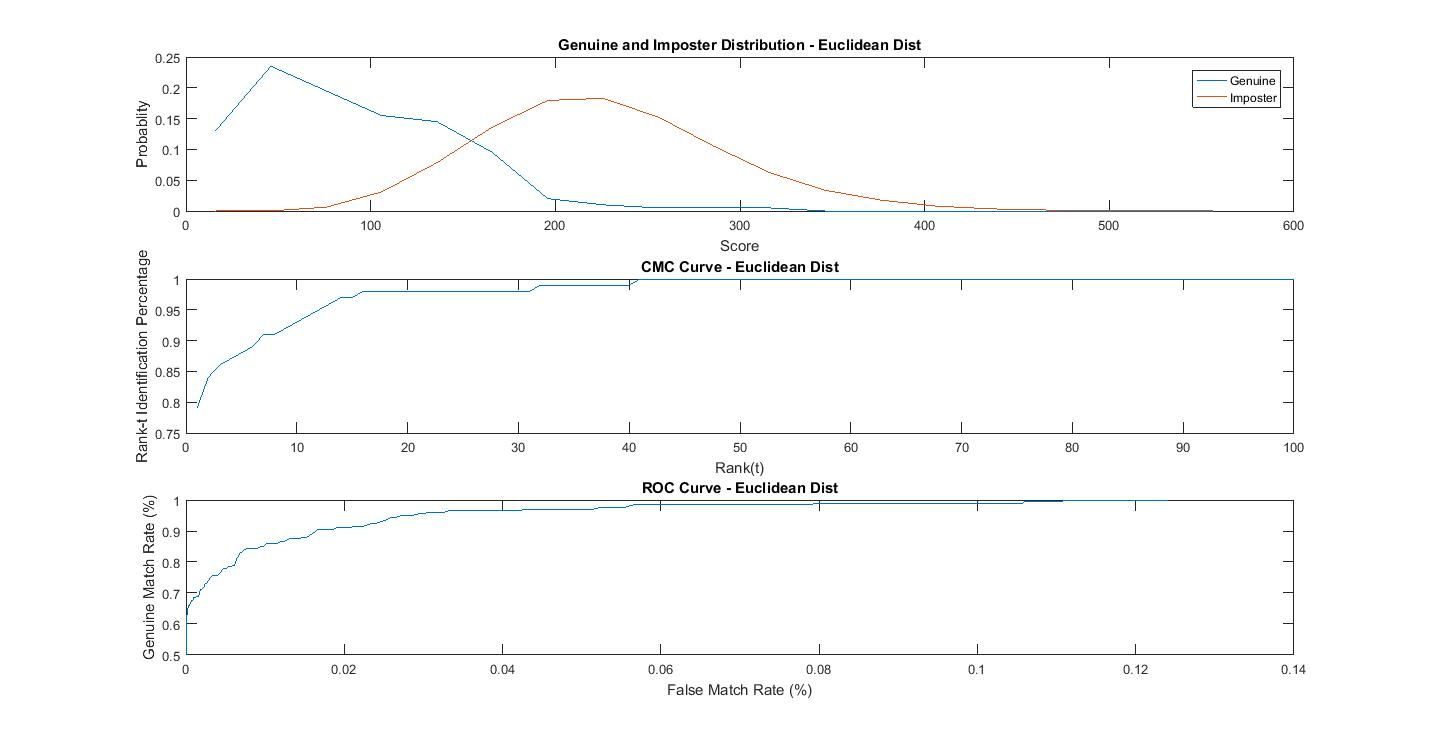
\includegraphics[width=20cm]{forTop70Coefficients.jpg}
\caption{The Performance Characteristics for top 70 Coefficients}
\label{top70Coef}
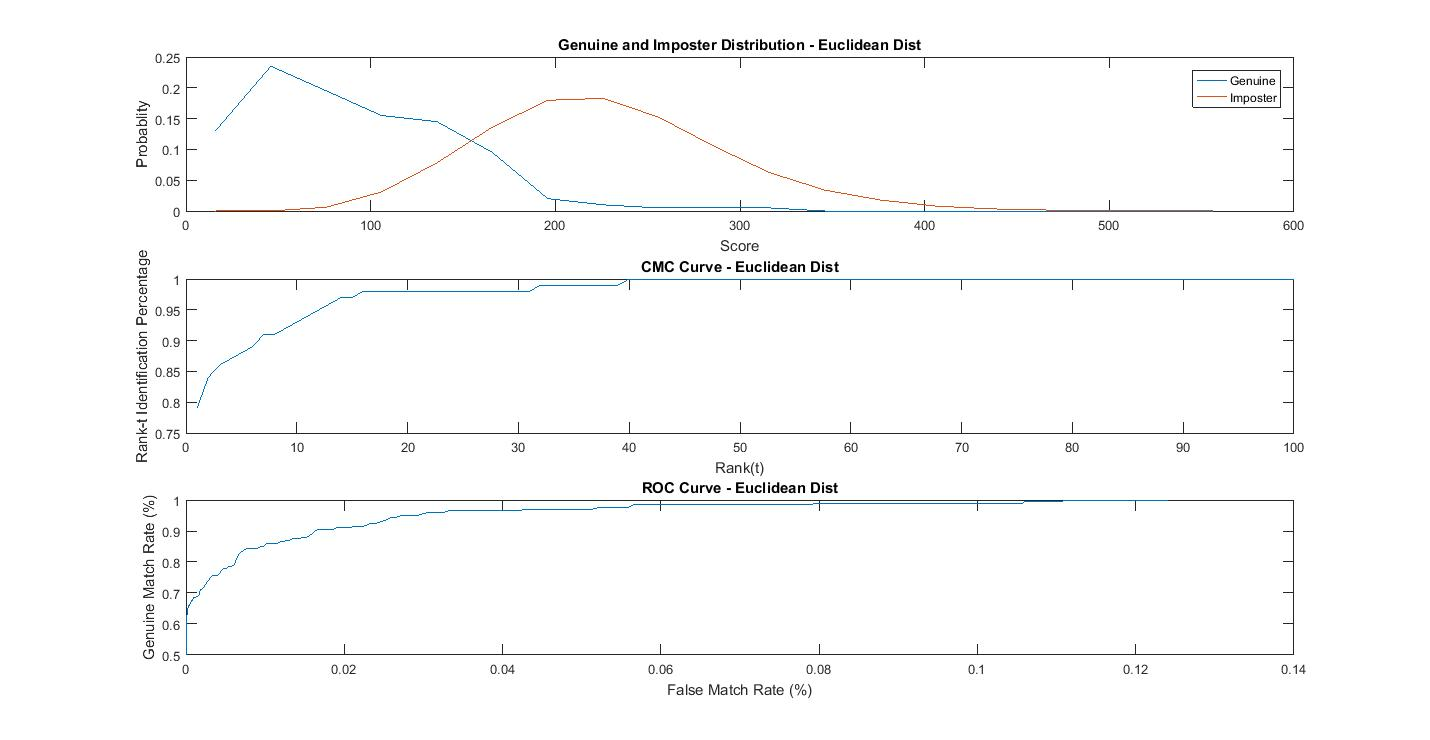
\includegraphics[width=20cm]{forTop80Coeffecients.jpg}
\caption{The Performance Characteristics for top 80 Coefficients}
\label{top80Coef}
\end{figure*}

\begin{figure*}
\centering
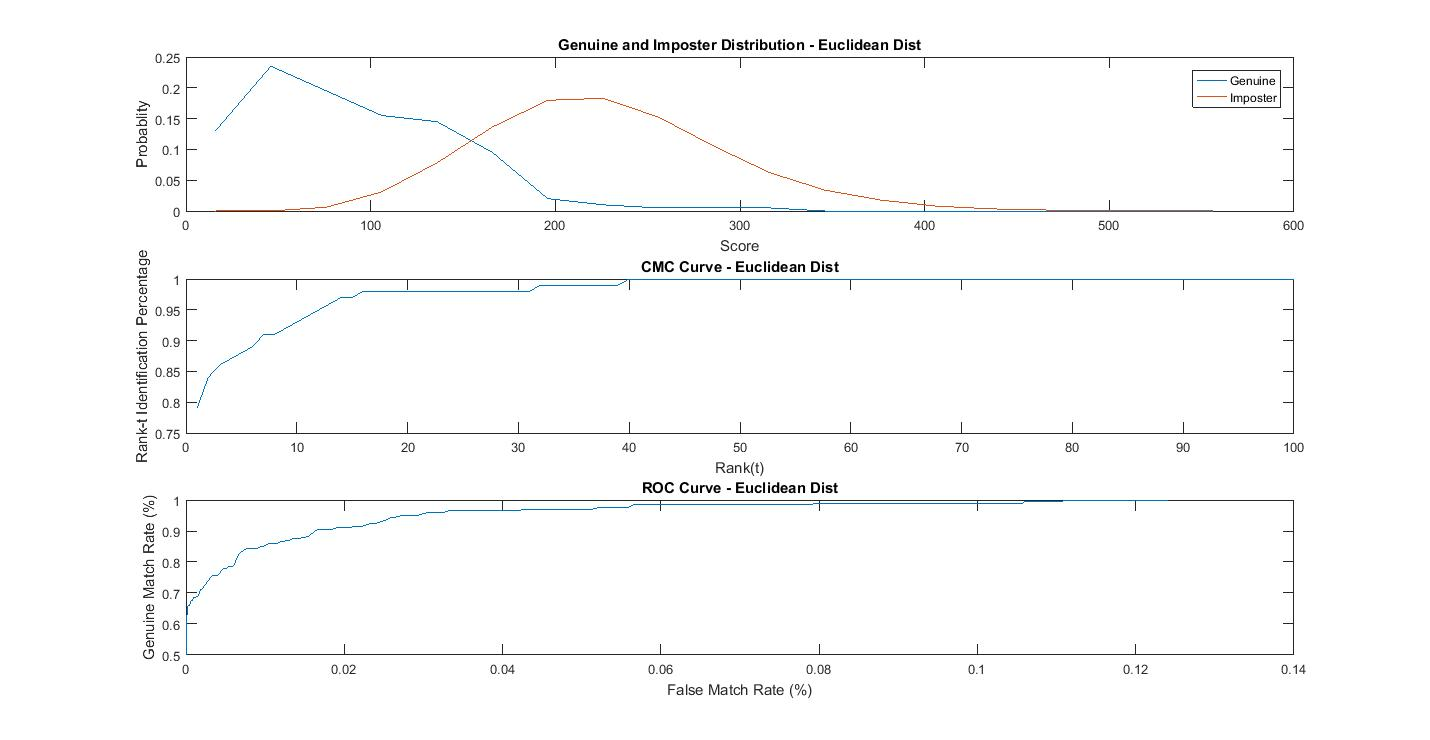
\includegraphics[width=20cm]{forTop90Coeffecients.jpg}
\caption{The Performance Characteristics for top 90 Coefficients}
\label{top90Coef}
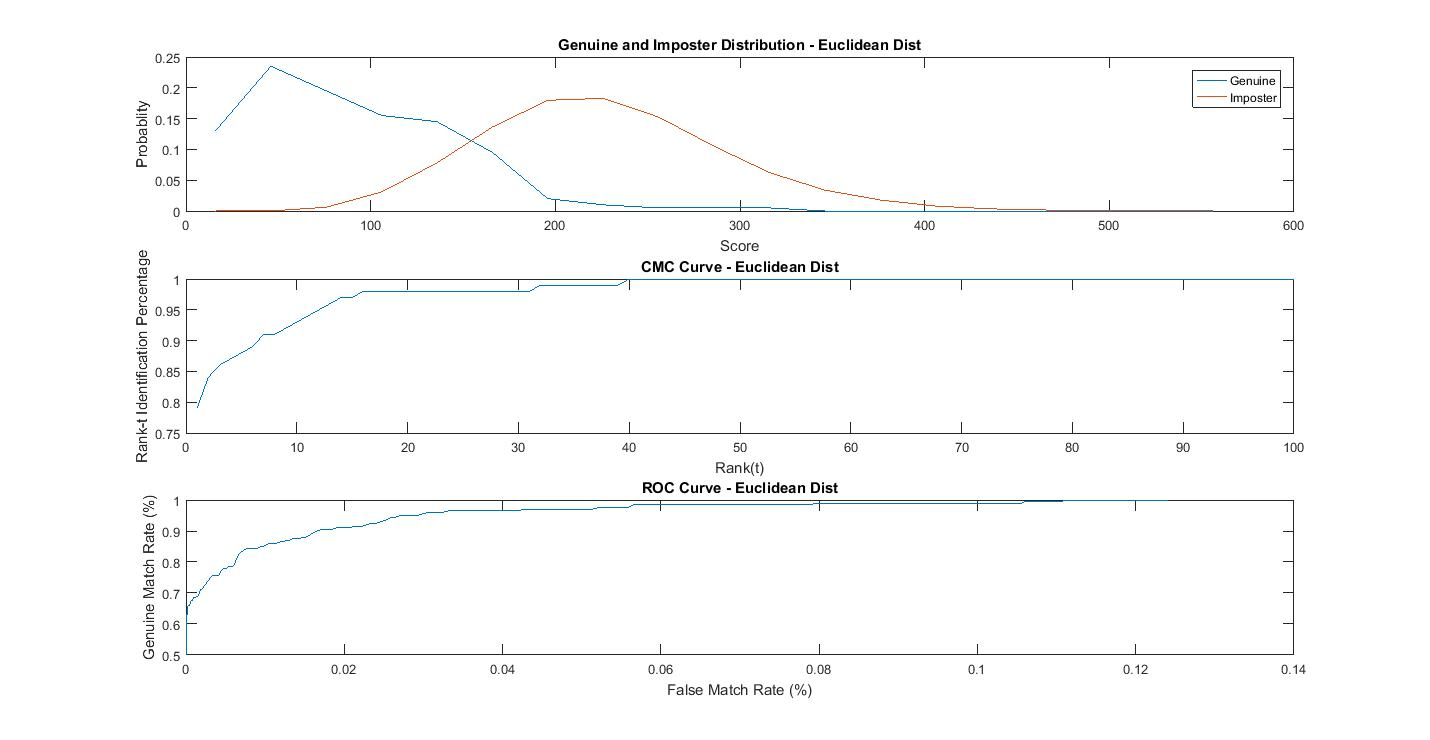
\includegraphics[width=20cm]{forTop100Coeffecients.jpg}
\caption{The Performance Characteristics for top 100 Coefficients}
\label{top100Coef}
\end{figure*}

\item Increasing the number of coefficients beyond this is not going to increase the performance of the system as we can see the recognition rate has leveled after 60 coefficients. This leads us to assume that most of the information is contained in the top 60 eigenvectors.


\item Using euclidean distance as a measure of similarity, we calculate the similarity matrix between the probe and the gallery images directly without reducing the dimensionality. The performance of this system is available in the figure \ref{withoutPCA}. By comparing the figure \ref{withoutPCA} and the characteristics for the system with PCA, we can clearly see that the area shared under the genuine and imposter is lesser for the system without the PCA, the area under the ROC curve is more for the system without PCA. From this we can infer that the system without PCA performs way better than the system with PCA. In this case using PCA reduces the performance of the system. There can be various reasons for this. Both the gallery and the probe data is perfectly normalized (which can never be achieved in the normal scenario). In case the images are not perfectly normalized we will get small variations in illumination and pose which can be overcome during recognition by using PCA. A similar case is explained in the \cite{PcaForFaceFirst}, where they use an approximation procedure to normalize the slight variations in the data. 
\begin{figure*}
\centering
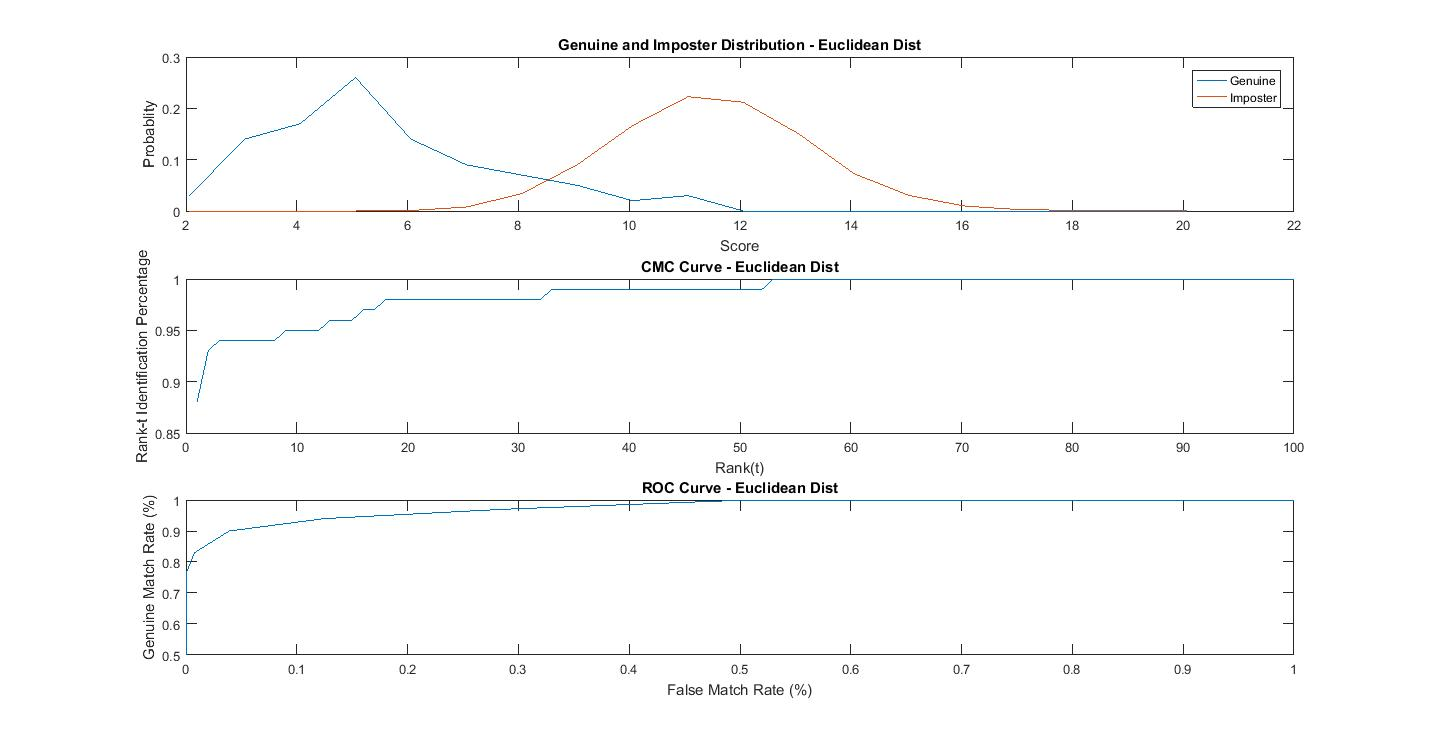
\includegraphics[width=20cm]{PerformanceWithoutPCA.jpg}
\caption{The performance Characteristics without PCA}
\label{withoutPCA}
\end{figure*}

\end{enumerate}
\textbf{K means}
\begin{enumerate}
\item We run the KMeans algorithm for different centroids. First we try it for the first 2 inputs from the dataset passed to the KMeans algorithm to get an accuracy of 57\% percentage. For the centroid seeded with zero mean we get an accuracy of 60.3\%. Thus we choose the zero mean as the standard seed for the rest of the experiments. 


\item By taking 10 to 100 coefficients( in steps of 10)  and euclidean distance as the distance measure we perform the K means algorithm to cluster the input data of total 300 images. The resultant clusters are validated for the different validity indices explained in the later poitns. Since using one criteria to measure the goodness of the cluster is not a good practice, we perform validation on various indices and try to analyze the data. 
\begin{figure*}
\centering
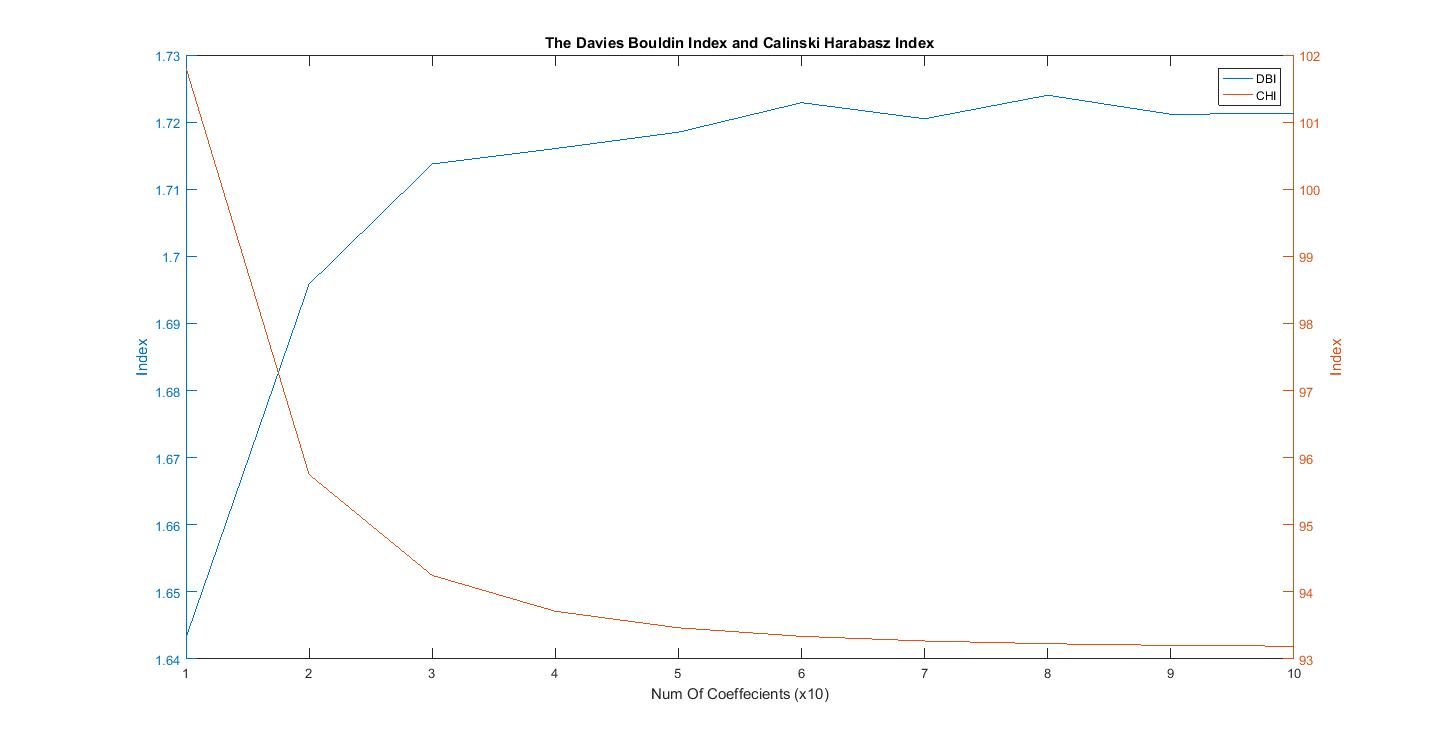
\includegraphics[width=20cm]{IndexVSNumberofCoeffecients.jpg}
\caption{Internal Validity Criteria vs Number of Coefficients}
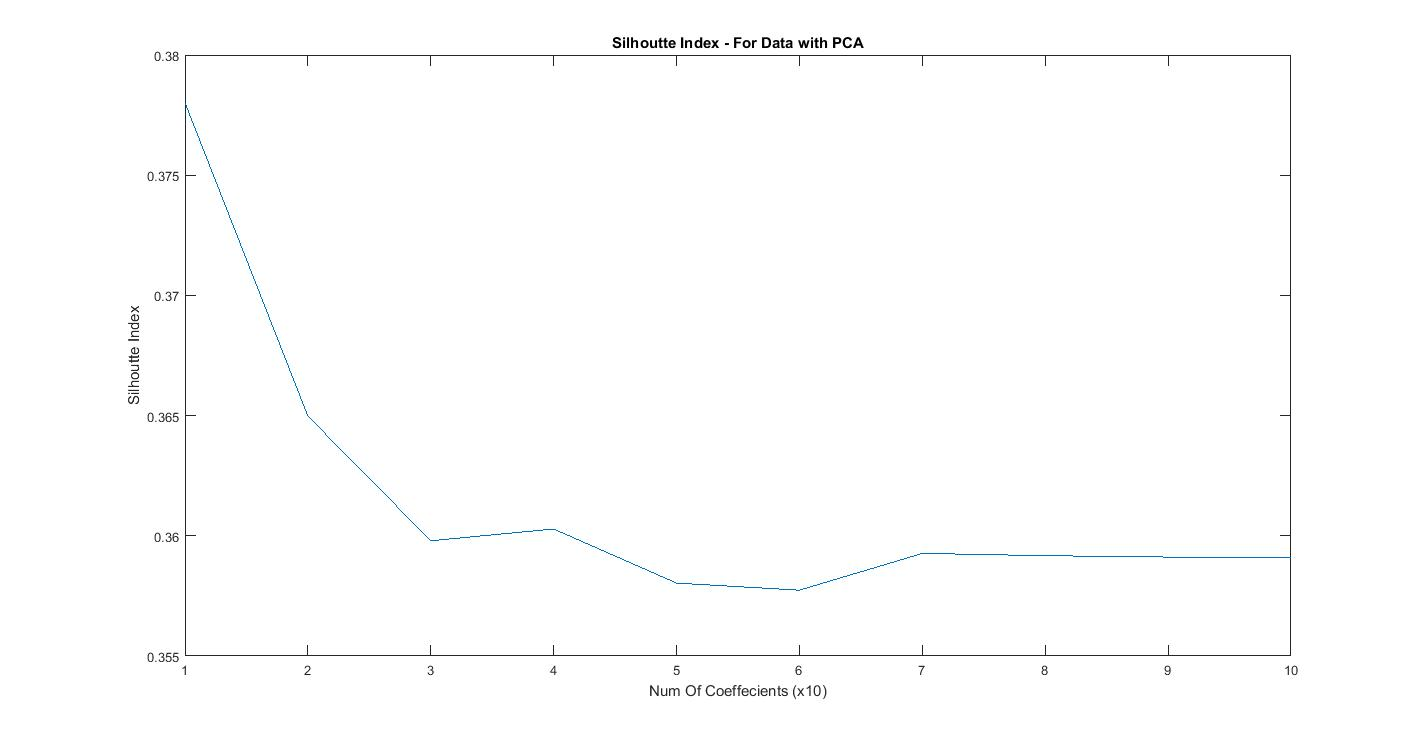
\includegraphics[width=20cm]{Silhoutte_Index}
\caption{Silhouette Index vs Number of Ceofficients}
\label{Internal}
\end{figure*}
\item The Internal criteria used for validation are Davies Bouldin Index(DB) and the  Calinski-Harabasz(CH) index. The plot of these two indices varying for different numbers of coefficients used is available in the figure \ref{Internal}. The number of coefficients that minimizes the DB index and the number of coefficients that maximizes the CH index is better. From the graph we can clearly get a winner the least number of coefficients show the best validity. But from both the curves we can see that they show a perfect cure either increasing or decreasing. So we check the performance with another index the silhouette index (available in the figure 21). From the three graphs we can find that the rate of change of the index is constant for number of coefficients at 20 and 30 hence leading us to infer that it would be the optimal number of coefficients. 
\begin{figure*}
\centering
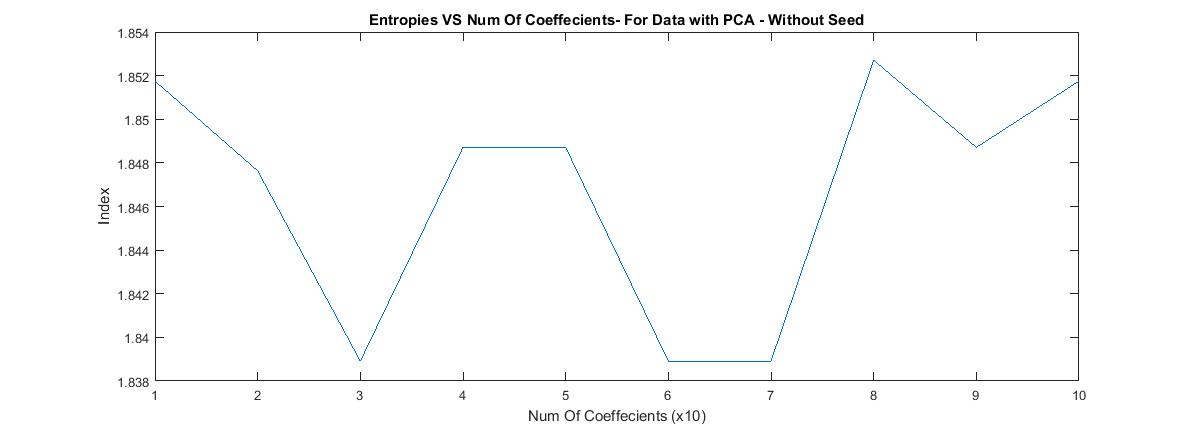
\includegraphics[width=20cm]{Entropies_withPCA_withoutSeed.jpg}
\caption{Entropy Validity Criteria - unseeded K mean}
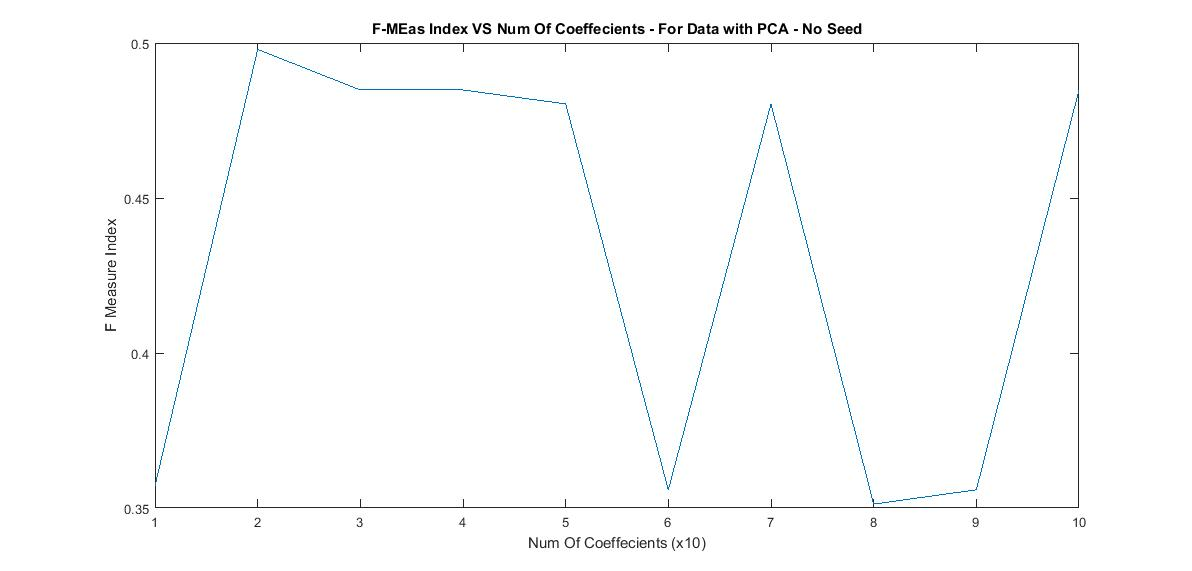
\includegraphics[width=20cm]{Fmeasure_withPCA_withoutSeed.jpg}
\caption{F1Measure Validity Criteria - unseeded K mean}
\label{External}
\end{figure*}
\begin{figure*}
\centering
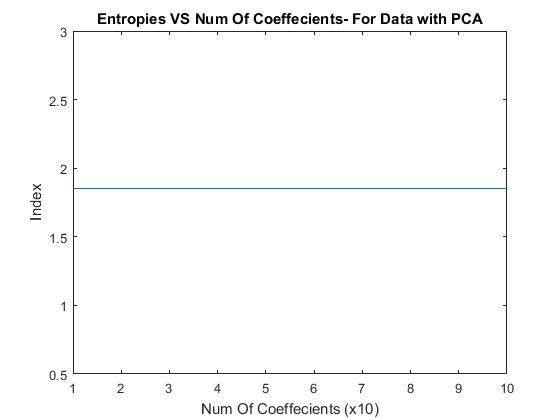
\includegraphics[height =10cm]{Entropies_withPCA_withSeed.jpg}
\caption{Entropy Validity Criteria - K Mean seeded with zero vector}
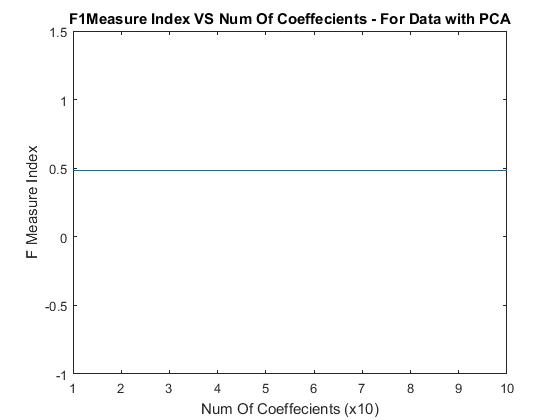
\includegraphics[height=10cm]{Fmeasure_withPCA_withSeed.jpg}
\caption{F1Measure Validity Criteria - K Mean seeded with zero vector}
\label{External2}
\end{figure*}

\item The External Criteria used for validation is Entropy and F1measure (fig \ref{External}).  Both measure almost similar properties of the cluster, true positives, true negatives, false positives and false negatives. From the figure \ref{External} we can see that the entropies are not constant and we repeat the step with K mean seeded with zero vector to obtain figure \ref{External2}. From the this fig \ref{External2}, we can see that the validity remains constant for the various number of coefficients. This leads us to understand that the PCA does not have any effect on the clustering. The accuracy of the system also remains around 60.30\%. This proves that the PCA has no effect on the clustering. This was clearly not visible in the internal criteria because the internal criteria did not take into account the actual labels of the data. In our case we have the external validity criteria(labels of the data)  and hence a more exact measure of the goodness is calculated in this case. 
\item Clustering the data without applying PCA also results in an approximately same accuracy 60\%. Thus we can confirm that PCA does not affect clustering of the data for soft biometrics.  

%\item This trend is not the same as in the recognition section. We can clearly see that increasing the components increase the rank1 recognition rate. But increasing the components for clustering does not change the performance.

\end{enumerate}
% An example of a floating figure using the graphicx package.
% Note that \label must occur AFTER (or within) \caption.
% For figures, \caption should occur after the \graphics.
% Note that IEEEtran v1.7 and later has special internal code that
% is designed to preserve the operation of \label within \caption
% even when the captionsoff option is in effect. However, because
% of issues like this, it may be the safest practice to put all your
% \label just after \caption rather than within \caption{}.
%
% Reminder: the "draftcls" or "draftclsnofoot", not "draft", class
% option should be used if it is desired that the figures are to be
% displayed while in draft mode.
%
%\begin{figure}[!t]
%\centering
%\includegraphics[width=2.5in]{myfigure}
% where an .eps filename suffix will be assumed under latex, 
% and a .pdf suffix will be assumed for pdflatex; or what has been declared
% via \DeclareGraphicsExtensions.
%\caption{Simulation results for the network.}
%\label{fig_sim}
%\end{figure}

% Note that the IEEE typically puts floats only at the top, even when this
% results in a large percentage of a column being occupied by floats.


% An example of a double column floating figure using two subfigures.
% (The subfig.sty package must be loaded for this to work.)
% The subfigure \label commands are set within each subfloat command,
% and the \label for the overall figure must come after \caption.
% \hfil is used as a separator to get equal spacing.
% Watch out that the combined width of all the subfigures on a 
% line do not exceed the text width or a line break will occur.
%
%\begin{figure*}[!t]
%\centering
%\subfloat[Case I]{\includegraphics[width=2.5in]{box}%
%\label{fig_first_case}}
%\hfil
%\subfloat[Case II]{\includegraphics[width=2.5in]{box}%
%\label{fig_second_case}}
%\caption{Simulation results for the network.}
%\label{fig_sim}
%\end{figure*}
%
% Note that often IEEE papers with subfigures do not employ subfigure
% captions (using the optional argument to \subfloat[]), but instead will
% reference/describe all of them (a), (b), etc., within the main caption.
% Be aware that for subfig.sty to generate the (a), (b), etc., subfigure
% labels, the optional argument to \subfloat must be present. If a
% subcaption is not desired, just leave its contents blank,
% e.g., \subfloat[].


% An example of a floating table. Note that, for IEEE style tables, the
% \caption command should come BEFORE the table and, given that table
% captions serve much like titles, are usually capitalized except for words
% such as a, an, and, as, at, but, by, for, in, nor, of, on, or, the, to
% and up, which are usually not capitalized unless they are the first or
% last word of the caption. Table text will default to \footnotesize as
% the IEEE normally uses this smaller font for tables.
% The \label must come after \caption as always.
%
%\begin{table}[!t]
%% increase table row spacing, adjust to taste
%\renewcommand{\arraystretch}{1.3}
% if using array.sty, it might be a good idea to tweak the value of
% \extrarowheight as needed to properly center the text within the cells
%\caption{An Example of a Table}
%\label{table_example}
%\centering
%% Some packages, such as MDW tools, offer better commands for making tables
%% than the plain LaTeX2e tabular which is used here.
%\begin{tabular}{|c||c|}
%\hline
%One & Two\\
%\hline
%Three & Four\\
%\hline
%\end{tabular}
%\end{table}


% Note that the IEEE does not put floats in the very first column
% - or typically anywhere on the first page for that matter. Also,
% in-text middle ("here") positioning is typically not used, but it
% is allowed and encouraged for Computer Society conferences (but
% not Computer Society journals). Most IEEE journals/conferences use
% top floats exclusively. 
% Note that, LaTeX2e, unlike IEEE journals/conferences, places
% footnotes above bottom floats. This can be corrected via the
% \fnbelowfloat command of the stfloats package.




\section{Conclusion}

\begin{enumerate}

\item The top 3 eigen faces are available in figure \ref{fig:top3}. The first principal component in terms of facial component corresponds to illumination invariance.
\item The recognitionperformance does not vary after an initial increase in performance
\item The PCA does not have an effect on the clustering. 
\end{enumerate}

% conference papers do not normally have an appendix


% use section* for acknowledgment






% trigger a \newpage just before the given reference
% number - used to balance the columns on the last page
% adjust value as needed - may need to be readjusted if
% the document is modified later
%\IEEEtriggeratref{8}
% The "triggered" command can be changed if desired:
%\IEEEtriggercmd{\enlargethispage{-5in}}

% references section

% can use a bibliography generated by BibTeX as a .bbl file
% BibTeX documentation can be easily obtained at:
% http://mirror.ctan.org/biblio/bibtex/contrib/doc/
% The IEEEtran BibTeX style support page is at:
% http://www.michaelshell.org/tex/ieeetran/bibtex/
%\bibliographystyle{IEEEtran}
% argument is your BibTeX string definitions and bibliography database(s)
%\bibliography{IEEEabrv,../bib/paper}
%
% <OR> manually copy in the resultant .bbl file
% set second argument of \begin to the number of references
% (used to reserve space for the reference number labels box)
\begin{thebibliography}{1}

\bibitem{AJain-one}
A. K. Jain, A. Ross and S. Prabhakar, "An introduction to biometric recognition," in IEEE Transactions on Circuits and Systems for Video Technology, vol. 14, no. 1, pp. 4-20, Jan. 2004.
doi: 10.1109/TCSVT.2003.818349

\bibitem{PcaForFaceFirst}
 Sirovich and Kirby "Low Dimensonal Procedure for Characterisation of Human Faces" (1987)
 
 \bibitem{BishopPattern}
 Bishop, Christopher M. "Pattern recognition." Machine Learning 128 (2006).
APA	


\end{thebibliography}

  


% that's all folks
\end{document}


